\documentclass[12pt]{article}
\usepackage{comment}
\usepackage{listings}
\usepackage{enumitem}
\usepackage[utf8x]{inputenc}
\usepackage[catalan]{babel}
\usepackage{graphicx}
\usepackage{wrapfig}
\usepackage{booktabs}
\usepackage{hyperref}
\hypersetup{
    colorlinks=true,
    linkcolor=black,
    filecolor=magenta,      
    urlcolor=cyan,
}

\graphicspath{ {images/} }
\usepackage{geometry}
 \geometry{
 a4paper,
 total={170mm,257mm},
 left=25mm,
 top=25mm,
 bottom=25mm
 }
 
 \usepackage[most]{tcolorbox}
\newtcolorbox{myframe}[1][]{
  enhanced,
  arc=0pt,
  outer arc=0pt,
  colback=white,
  boxrule=0.8pt,
  #1
}
 


\begin{document}

\begin{titlepage}

\begin{center}
\vspace*{1in}
\begin{figure}[htb]
\begin{center}

\includegraphics[width=5cm]{logo}
\end{center}
\end{figure}

PARADIGMES I LLENGUATGES DE PROGRAMACIÓ
\vspace*{0.15in}
\vspace*{0.6in}
\begin{large}
\\
\end{large}
\vspace*{0.2in}
\begin{Large}
\textbf{PRÀCTICA DE HASKELL} \\
\end{Large}
\vspace*{0.2in}
\begin{large}
Validador de jugades d'escacs\\
\end{large}
\vspace*{0.2in}
\rule{80mm}{0.1mm}\\
\vspace*{0.2in}
\begin{large}
Jose Garvin Victoria \\
Mauro Balestra Sastriques \\
\vspace*{0.2in}
 \textbf{Enginyeria informàtica}\\
 \vspace*{0.2in}
 \textbf{Curs 2018/19}
\end{large}
\end{center}

\end{titlepage}



\newpage
\tableofcontents

\newpage
\section{Introducció i abast}

\subsection{Introducció i objectiu}
L'objectiu d'aquesta pràctica és l'implementació d'un validador de jugades d'escacs en el llenguatge de programació \textbf{Haskell}. \\
El funcionament principal d'aquest programa és divideix en els següents blocs:
\begin{itemize}
\item Interacció amb l'usuari per demanar el fitxer de text amb les jugades de la partida d'escacs. 
\item Lectura del fitxer de text, on assumim que el format és correcte i que la notació emprada és la \href{https://ca.wikipedia.org/wiki/Notaci%C3%B3_algebraica}{\textbf{algebraica estesa}}.
\item Per cada jugada llegida del fitxer, es generen unes jugades on es validarán la seva correctesa, amb indicació de captures, escacs i escac i mat.
\item Per pantalla es mostraràn els estats de la partida en curs, fins arribar al final, on trobarem un missatge indicant el guanyador, si n'hi ha, empat, o bé un missatge d'error indicant quina ha estat la jugada invàlida.
\end{itemize}

\subsection{Abast de la pràctica}

Per problemes de sintaxi i comprensió del paradigma de programació, l'abast ha estat fins a la nota de 8:
\\
\\
\noindent
\textit{Compliments i notes: \\
- Fins a un 8. Validació de notació correcta (amb indicació de captures, escacs i escac i mat), de moviments correctes (sense controlar captura al pas, coronació i enrocs), detecció d’escac i mat, representació textual i interacció amb l’usuari correcte}
\\
\\
\noindent
Cal dir que encara que el grup no ha pogut assolir l'objectiu de l'abast de puntuació de 10, s'ha pogut acurar el disseny del programa, emprant mòduls (no programar tot en un sol fitxer), llistes per comprhensió, i funcions d'ordre superior a la majoria de mètodes \textbf{importants} del programa. 
\\
\\
Gairebé no s'han hagut d'importar mòduls externs de la distribució GHC, ja que creiem que era millor aprendre a implementar aquestes funcions que ens oferia aquesta distribució pel nostre compte, per tal d'adquirir els coneixements adequats d'aquest paradigma.


\section{Resolució del problema}

Com a part de resolució del problema, el més important, ha estat pensar molt bé quins serien els tipus a implementar del validador d'escacs. En aquest apartat ens centrarem en explicar quins han estat els tipus de dades que hem utilitzat i que creiem que cal destacar i quines són les funcions del nostre programa que considerem més importants, i dignes de comentar.
\\
\\
Dividirem aquesta secció en 3 apartats; en un d'ells parlarem sobre els tipus utilitzats, en un altre comentarem les funcions que creiem més importants i que pensem que hem d'explicar clarament perque s'entengui millor el codi i per últim, un apartat on comentarem altres aspectes importants del nostre codi que pensem que són convenients d'explicat amb detall.




\subsection{Definicions de tipus}

En aquest apartat llistarem quins són el tipus que hem definit per a poder desenvolupar la pràctica i explicarem la finalitat per a la qual s'ha decidit definir cadascun dels tipus:
\noindent
\\
\\
Al fitxer \textbf{"Jugada.hs"} hem definit els següents tipus:
\begin{itemize}
\item \textsf{data Jugada = Jugada {tipusPeca :: Peca, origen :: Posicio, desti :: Posicio, accio :: Accio} $|$ Acabada deriving (Eq)}: Aquest tipus l'utilitzem per representar jugades al joc d'escacs. Una jugada la representem a partir d'una peça, una posició origen, una posició destí, i una acció a realitzar. Aquest tipus deriva de la classe \textit{Equals}, aixó ens permetra poder comparar taulers.
\end{itemize}

\begin{itemize}
\item \textsf{data Accio = Matar $|$ Escac $|$ EscacIMat $|$ Res deriving (Eq)}: Aquest tipus l'utilitzem per representar jugades al joc d'escacs. Una jugada la representem a partir d'una peça, una posició origen, una posició destí, i una acció a realitzar. Aquest tipus deriva de la classe \textit{Equals}, aixó ens permetra poder comparar accions.
\end{itemize}


\noindent
\\
\\
Al fitxer \textbf{"Partida.hs"} hem definit els següents tipus:
\begin{itemize}
\item \textsf{data Partida = Partida Tauler Torn deriving (Eq)}: Aquest tipus l'utilitzem per representar partides al joc d'escacs. Una partida la representem a partir d'un tauler i una acció.
\end{itemize}



\noindent
\\
\\
Al fitxer \textbf{"Peca.hs"} hem definit els següents tipus:
\begin{itemize}
\item \textsf{data Peca = Peca { tipus::TipusPeca, color::ColorPeca } $|$ Buida deriving (Eq)}: Aquest tipus l'utilitzem per representar peces al joc d'escacs. Ens ha estat necessari definir peces de tipus \textit{Buida}. Si una peça no es \textit{Buida}, estarà representada a partir d'un tipus de peça i un color (blanc i negre). Aquest tipus deriva de la classe \textit{Equals}, aixó ens permetra poder comparar peces durant el desenvolupament d'una partida.
\end{itemize}

\begin{itemize}
\item \textsf{data TipusPeca = Peo $|$ Cavall $|$ Alfil $|$ Torre $|$ Dama $|$ Rei deriving (Read)}: Aquest tipus l'utilitzem per representar el tipus d'una  al joc d'escacs. Aquest tipus podrà ser peó, cavall, alfil, torre, dama o rei. Hem fet que aquest tipus derivi de la classe \textit{Read}, aixó ens permetra poder llegir tipus de peces.
\end{itemize}

\begin{itemize}
\item \textsf{data ColorPeca = Blanc | Negre | NoColor deriving (Eq, Show, Read)}: Aquest tipus l'utilitzem per representar el color d'una peça. Ens ha estat necessari definir un color de peça de tipus \textit{NoColor}. Hem fet que aquest tipus derivi de la classe \textit{Read},  \textit{Eq}, \textit{Show} aixó ens permetra poder llegir colors de peça, comparar-los i mostrar-los.
\end{itemize}


\noindent
\\
\\
Al fitxer \textbf{"Tauler.hs"} hem definit els següents tipus:
\begin{itemize}
\item \textsf{data Tauler = Tauler LlistaParell deriving (Eq)}: Aquest tipus l'utilitzem per representar partides el tauler d'escacs. Hem decidit representar el tauler utilitzant un tipus creat per nosaltres, que hem anomenat \textit{LlistaParell}. Es pot veure com s'ha implementat aquest tipus a l'arxiu \textbf{"Tauler.hs"}. El nostre tauler deriva de la classe \textit{Eq} aixó ens permetrà poder comparar taulers.
\end{itemize}

\subsection{Funcions a destacar}
En aquest apartat explicarem quin es el comportament de les funcions que creiem que cal destacar per tal d'entendre el funcionament del nostre validador d'escacs. Explicar cadascuna de les funcions faria que aquest document fós massa extens i per tant ens limitarem a explicar les funcions que creiem que són més rellevants.

\begin{itemize}
\item Funció \textit{moviment} : Aquesta funció rep una Peça, i una posició, i retorna totes les posicions que pot fer la peça en qüestió en un tauler buit.

\begin{figure}[htb]
\begin{center}
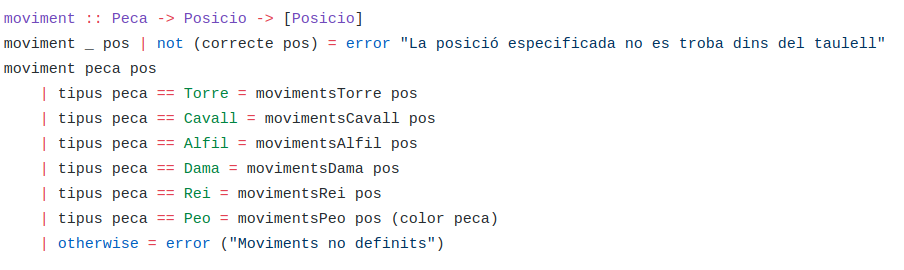
\includegraphics[width=17cm]{funcio_moviment}
\end{center}
\end{figure}

\item Funció \textit{movimentsRei} : Aquesta funció es específica pels moviments del Rei, es realitza un filter sobre tots els moviments de la Dama, filtrant tots els moviments que siguin més grans a 1. Per tant es queda amb totes les posicions disponibles amb distància <= 1.

\begin{figure}[htb]
\begin{center}
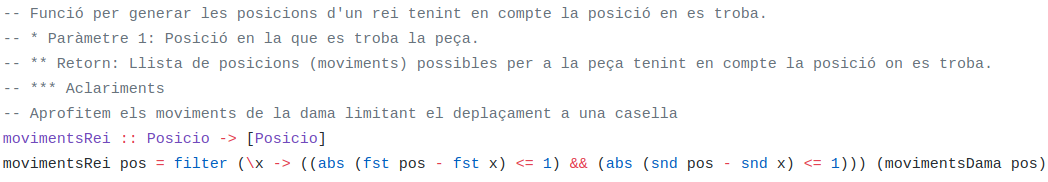
\includegraphics[width=18cm]{movimentsRei}
\end{center}
\end{figure}

\item Funció \textit{escac} : Donat l'estat actual del tauler, i un color de jugador, i indica si aquell bàndol ha rebut escac.

\begin{figure}[htb]
\begin{center}
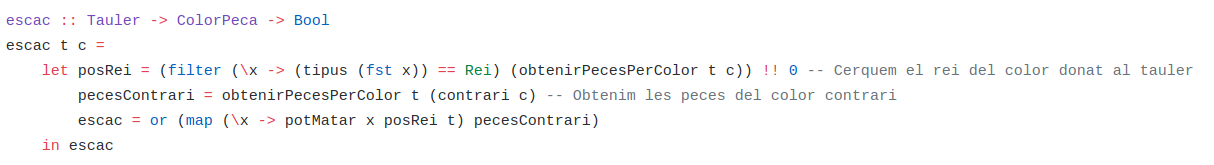
\includegraphics[width=18cm]{escac}
\end{center}
\end{figure}

\newpage

\item Funció \textit{escacIMat} : Donat l'estat actual del tauler, i un color de jugador, i indica si aquell bàndol ha rebut escac i mat, i per tant han perdut la partida.

\begin{figure}[htb]
\begin{center}
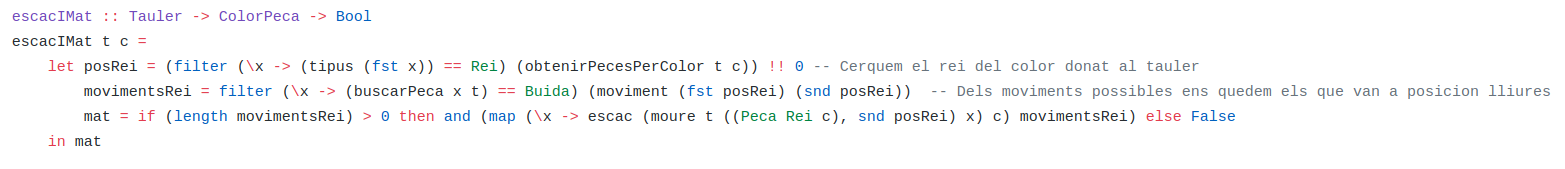
\includegraphics[width=18cm]{escacIMat}
\end{center}
\end{figure}

\item Funció \textit{fesJugada} : Aquesta és una de les funcions més importants, ja que comprova si la jugada que es va a realitzar es correcte, comprovant: La obligació de matar, comprovant que el contingut del fitxer es correspont amb el del tauler actual, indicant captures, escacs i escac i mat. Retorna un nou tauler amb la jugada feta, si es correcte.

\begin{figure}[htb]
\begin{center}
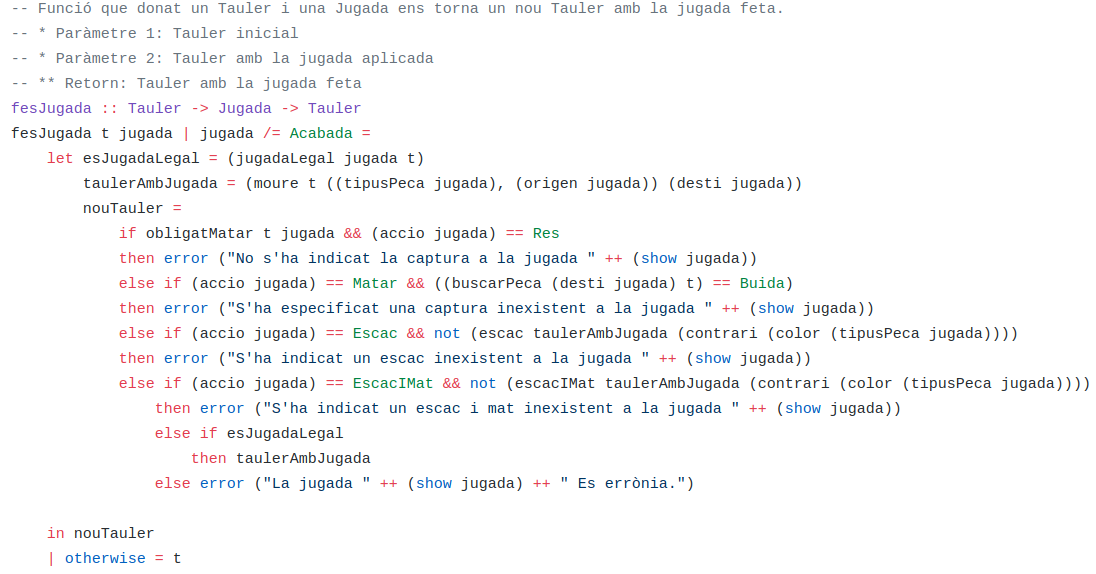
\includegraphics[width=17cm]{fesJugada}
\end{center}
\end{figure}

\item Funció principal \textit{main} : Funció principal d'entrada del programa, es crea la partida, mostrant el tauler inicial, i es van concatenant jugades dins una llista que després el mètode mostrarJoc, mostrarà.

\begin{figure}[htb]
\begin{center}
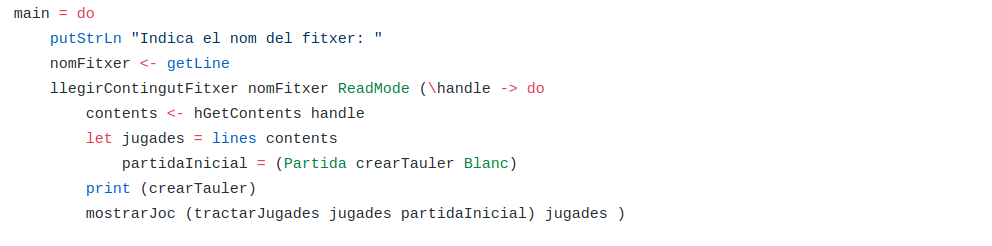
\includegraphics[width=18cm]{main}
\end{center}
\end{figure}

\end{itemize}

\newpage

\section{Execució i proves}
En aquest apartat del document explicarem com cal executar el nostre programa i mostrarem algunes de les sortides que hem obtingut pasant els fitxers de proves que s'ens han facilitat i altres fitxers de proves que hem creat nosaltres.

\subsection{Com executar}
Per tal d'executar el nostre programa caldrà tenir instal·lat l'intèrpret de Haskell GHCI. Un cop tinguem l'intèrpret instal·lat al nostre sistema i estem ubicats a la ruta on es troba el codi, podrem executar el programa fent servir l'instrucció que es mostra a continuació:

\begin{center}
\begin{lstlisting}[language=bash]
  $ runhaskell main.hs
\end{lstlisting}
\end{center}
\noindent
En executar el programa, haurem d'especificar la ruta a un fitxer d'entrada que haurà de seguir el format especificat en l'enunciat de la pràctica per tal de començar a utilitzar el nostre validador.

\subsection{Jocs de proves}
A continuació es mostren unes quantes sortides obtingudes al passar al nostre programa verificador de jugades d'escacs.
\\
\\
- \textbf{Sortida del test} \textit{pastor.txt} :
\begin{center}
\begin{lstlisting}[language=bash]
Indica el nom del fitxer: 
tests/pastor.txt
   ==========
8- |tcadract|
7- |pppppppp|
6- |........|
5- |........|
4- |........|
3- |........|
2- |PPPPPPPP|
1- |TCADRACT|
   ==========
    abcdefgh 

Tirada 1. Pe2e4 Pe7e5
   ==========
8- |tcadract|
7- |pppp.ppp|
6- |........|
5- |....p...|
4- |....P...|
3- |........|
2- |PPPP.PPP|
1- |TCADRACT|
   ==========
    abcdefgh 

Tirada 2. Af1c4 Cb8c6
   ==========
8- |t.adract|
7- |pppp.ppp|
6- |..c.....|
5- |....p...|
4- |..A.P...|
3- |........|
2- |PPPP.PPP|
1- |TCADR.CT|
   ==========
    abcdefgh 

Tirada 3. Dd1h5 Cg8f6
   ==========
8- |t.adra.t|
7- |pppp.ppp|
6- |..c..c..|
5- |....p..D|
4- |..A.P...|
3- |........|
2- |PPPP.PPP|
1- |TCA.R.CT|
   ==========
    abcdefgh 

Tirada 4. Dh5xf7++
   ==========
8- |t.adra.t|
7- |pppp.Dpp|
6- |..c..c..|
5- |....p...|
4- |..A.P...|
3- |........|
2- |PPPP.PPP|
1- |TCA.R.CT|
   ==========
    abcdefgh 

Fi de partida, blanques guanyen!!!
\end{lstlisting}
\end{center}


\newpage 
\noindent
- \textbf{Sortida del test} \textit{pastor.txt} :

\begin{center}
\begin{lstlisting}[language=bash]
Indica el nom del fitxer: 
tests/obligar_matar.txt
   ==========
8- |tcadract|
7- |pppppppp|
6- |........|
5- |........|
4- |........|
3- |........|
2- |PPPPPPPP|
1- |TCADRACT|
   ==========
    abcdefgh 

Tirada 1. Pd2d4 Pe7e5
   ==========
8- |tcadract|
7- |pppp.ppp|
6- |........|
5- |....p...|
4- |...P....|
3- |........|
2- |PPP.PPPP|
1- |TCADRACT|
   ==========
    abcdefgh 

Tirada 2. Pd4d5 
main.hs: No s'ha indicat la captura a la jugada amb peca (P) 
, posicio origen (4,4), posicio desti (4,5) i accio moure.
CallStack (from HasCallStack):
  error, called at ./Jugada.hs:124:18 in main:Jugada
\end{lstlisting}
\end{center}

\newpage


\section{Observacions}
Durant el desenvolupament d'aquesta pràctica hem asimilat molts aspectes que encara no teniem clar de la forma de programar amb Haskell. Tot i que podría semblar una pràctica simple de fer, utilitzant qualsevol altre paradigme de programació, al fer-ho amb Haskell ens hem anat trobant amb problemes que s'han pogut anar solucionant.
\\
\\
Considerem que en general la pràctica no es gaire complexa si només s'aspira a un 8, peró
 en el nostre cas, no hem pogut complir els altres objectius per falta de temps ja que els problemes esmentats anteriorment han requerit de temps per ser solucionats.
\\
\\
En resum, ens ha agradat fer aquesta pràctica, perquè hem pogut asimilar conceptes sobre el funcionament d'aquest llenguatge de programació que pensàvem que teniem controlats, pero a l'hora de la veritat ens hem adonat que no, ja que programar utilitzant aquest paradigma requereix un canvi de mentalitat bastant gran.

\newpage
\section{Bibliografía}

\setitemize{labelindent=-2em,labelsep=1cm,leftmargin=*}
\begin{itemize}[label={}]

\item Aprende Haskell: \url{http://aprendehaskell.es/main.html}
\item How work on lists: \url{https://wiki.haskell.org/How_to_work_on_lists}
\item Let vs. where: \url{https://wiki.haskell.org/Let_vs._Where}
\item Files: \url{https://www.glc.us.es/~jalonso/vestigium/i1m2016-manejo-de-ficheros-en-haskell/}
\item Substring: \url{https://rosettacode.org/wiki/Substring#Haskell}
\item Data type: \url{http://aprendehaskell.es/content/ClasesDeTipos.html#introduccion-a-los-tipos-de-datos-algebraicos}

\end{itemize}

\end{document}
